  \chapter{Research Methodologies}

\begin{greybox}

\textbf{Changes Needed for Assignment 3}

\vspace{1em}

\small
\renewcommand{\arraystretch}{1.3}

\begin{tabularx}{\linewidth}{
  |>{\raggedright\arraybackslash}X
  |>{\centering\arraybackslash}p{0.9cm}
  |>{\centering\arraybackslash}p{1.4cm}|
}
\hline
\textbf{Task} & \textbf{Done} & \textbf{Owner} \\
\hline

\parbox[t]{\linewidth}{
  \textbf{Title}

  Description
}
& $\square$ & \\ 
\hline

\parbox[t]{\linewidth}{
  \textbf{Title}

  Description
}
& $\square$ & \\ 
\hline

\parbox[t]{\linewidth}{
  \textbf{Title}

  Description
}
& $\square$ & \\ 
\hline

\end{tabularx}

\end{greybox}


  \section{Proposed Framework}

  DANES~\citep{truica2024danes} and GETAE~\citep{GETAE2025} classify inauthentic social media content by fusing a single-modal text-based content branch and a social context branch to create an ensemble model. The proposed MACE (\textbf{M}ultimodal \textbf{A}nd \textbf{C}ontext-aware \textbf{E}nsemble) framework adopts a comparative experimental design to evaluate the impact of integrating multimodal content features into these models.

  MACE retains the dual-branch structure and social context features of DANES and GETAE, and replaces the text-based content branch with a multimodal content branch, allowing for evaluation of the classification performance of multimodal content features within these ensemble frameworks.

  \begin{figure}[H]
      \centering
      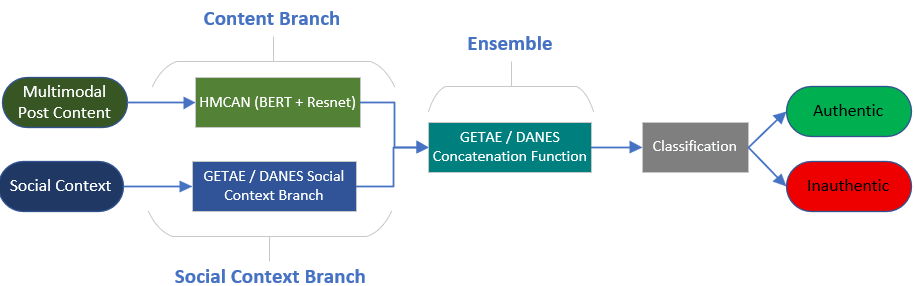
\includegraphics[width=0.95\textwidth]{figs/MACE-Architecture}
      \caption{
      Proposed MACE Ensemble Framework for Inauthentic Social Media Post Classification
      }
      \label{fig:MACE-Architecture}
  \end{figure}



\subsection{Multimodal Content Branch}

MACE adopts HMCAN (Hierarchical Multimodal Contextual Attention Network) as the multimodal content branch \citep{Qian2021}. HMCAN is selected because it is task-aligned with multimodal fake news detection, has demonstrated strong performance on Twitter-based multimodal datasets, and uses an encoding pipeline that is compatible with the textual and visual components of the proposed datasets.

HMCAN extracts textual features using BERT and visual features using a pre-trained ResNet50 image encoder. These modality-specific representations are then passed through multimodal contextual attention and hierarchical encoding components to produce a single fixed-length post representation. For posts without attached images, HMCAN uses dummy images as visual placeholders to preserve data alignment \citep{Qian2021}. This makes HMCAN suitable for MACE because its output can serve as an architectural replacement for the text-only content embedding used in the original DANES/GETAE-style ensemble, while still supporting datasets that contain a mixture of image-containing and text-only posts.

In MACE, the HMCAN representation will be used as the content-branch embedding and concatenated with the existing social-context embedding before classification. If the HMCAN output dimension differs from the expected DANES/GETAE content-embedding dimension, a linear projection layer will be used as an adapter to map the HMCAN representation to the required size before concatenation.

This design allows the experiment to isolate the effect of substituting a multimodal content branch for the original text-only content branch while keeping the social-context branch, fusion mechanism, and classifier structure unchanged. As a result, any performance difference between the baseline and MACE conditions can be attributed primarily to the richer multimodal content representation rather than to simultaneous changes in downstream fusion or classification.

  \subsection{Social Context Branch}

  % Describe the user-level, interaction-based, and lightweight network/context features.
  We retain the Graph-based Deep Learning social context branches from the baseline DANES/GETAE architectures, as these studies and others provide strong evidence supporting the effectiveness of propagation and interaction signals in misinformation detection \citep{truica2024danes, GETAE2025, Song2021,Min2022,Zhu24}.

  \begin{table}[h]
  \centering
  {\small

  \begin{tabular}{lp{4.5cm}p{4.5cm}}
  \hline
  & \textbf{DANES} & \textbf{GETAE} \\
  \hline

  Social context approach & Graph embedding from static
    network structure &
    GNN over dynamic propagation graph \\
  Key information used & User interactions, relationships,
    and post behaviour &
    Information diffusion and propagation patterns \\
  \hline
  \end{tabular}
  \caption{Comparison of DANES and GETAE social context branches.}}
  \label{tab:danes_getae}

  \end{table}

\subsection{Feature Fusion and Classification}

Both fusion models combine branch outputs by concatenating the content and context embeddings to produce a single classification embedding. In DANES, this concatenated embedding is passed directly to a dense classification layer with softmax activation. In GETAE, the concatenated embedding is first passed through a dense hidden layer with ReLU activation, then through a final dense softmax classification layer. In both cases, the final softmax layer produces a probability distribution over the target classes and assigns the final label based on the highest predicted probability. MACE retains the classification mechanisms from the original frameworks.

The concatenation-based fusion mechanism is also retained in MACE. Multimodal fusion is a core design challenge in multimodal machine learning \citep{baltruvsaitis2019multimodal}. More recent work distinguishes between simple separate-encoder fusion, dedicated fusion networks, and unified cross-modal encoders, showing that fusion design can materially affect model behaviour and performance \citep{li2025multimodalalignment}.

More advanced fusion strategies may improve cross-modal interaction modelling. For example, MCAN argues that simple concatenation does not explicitly capture interdependence between text and image features, and instead proposes co-attention for multimodal fake news detection \citep{wu2021mcan}. Transformer-based fusion approaches also provide alternatives, including bottlenecked cross-modal attention mechanisms that aim to improve fusion performance while controlling computational cost \citep{nagrani2021attention}.

However, the objective of this study is not to optimise the fusion or classification mechanisms, but to isolate the effect of replacing the text-only content branch with a multimodal content branch in the DANES/GETAE-style ensemble, addressing limitations identified by \citet{Dellys2025}. Changes to these mechanisms would introduce additional confounding architectural variables. MACE therefore retains the existing concatenation-based fusion and classification mechanism so that observed performance differences can be attributed primarily to the content-branch substitution rather than to simultaneous changes in representation, fusion, and classification design.

  \section{Experimental Design}

  The experiment design is structured as a three-stage process to systematically evaluate dataset suitability, replicate the baseline architectures, and test the proposed MACE architecture. Both base architectures are evaluated so that findings can be assessed for consistency across the DANES and GETAE ensemble backbones.

  The model backbone is treated as a replication factor, rather than the primary independent variable, as the main focus is evaluating the impact of substituting the text-only content branch with a multimodal content branch. The research questions also require  assessment of dataset suitability and computational cost, so the experimental design includes a dataset adaptation and feasibility stage before full MACE evaluation.

  \subsection{Dataset Adaptation and Selection}

  Before Stage~3 model evaluation, candidate multimodal datasets will be assessed for compatibility with the MACE architecture. This stage addresses RQ3 by determining whether each dataset contains sufficient textual content, image availability, label compatibility, social-context or propagation information, and computational feasibility for use with the DANES/GETAE-style ensemble. Candidate datasets will be profiled for record count, image-availability rate, missing or broken media links, class balance, graph density, availability of user or propagation traces, and estimated storage and memory requirements.

  The dataset adaptation process will include preprocessing text fields, validating and downloading available images, creating dummy image placeholders where required, mapping dataset labels to the target classification structure, constructing or adapting social-context graph features, and producing dataset-level feasibility statistics. FakeNewsNet and MuMin will be considered as candidate Stage~2 datasets; however, final selection will depend on the adaptation results. Where more than one dataset satisfies the suitability criteria, MACE will be evaluated across multiple adapted datasets to assess generalisability. Where only one dataset is feasible within the available compute and time constraints, the excluded dataset characteristics and reasons for exclusion will be reported as part of the RQ3 findings.

  \subsection{Experiment Stages and Conditions}

  \textbf{Stage 1} replicates the published DANES and GETAE architectures and evaluates their performance on Twitter15 and Twitter16 to confirm that the implementation is consistent with the published baselines before introducing architectural modifications.

  \textbf{Stage 2} adapts candidate multimodal datasets and selects the dataset or datasets suitable for MACE evaluation. This stage establishes whether the available multimodal and social-context data can support the proposed experimental comparisons, and records dataset feasibility criteria relevant to RQ3.

  \textbf{Stage 3} evaluates four experimental conditions on the selected adapted multimodal dataset or datasets. Condition A establishes a dataset-specific baseline using the original text-only content branch and retained social-context branch. Conditions B, C, and D systematically evaluate the independent and combined contribution of text-only content, multimodal content, and social-context features.

  \begin{table}[h!]
  {\small
  \begin{tabular}{llllll}
  \hline
  \multicolumn{2}{l}{\textbf{Stage}} & \textbf{Label}                                                    & \textbf{\begin{tabular}[c]{@{}l@{}}Content\\ Branch\end{tabular}} & \textbf{\begin{tabular}[c]{@{}l@{}}Context\\ Branch\end{tabular}} & \textbf{Goal / Purpose}                                                                                                                          \\ \hline
  1                        & A       & \begin{tabular}[c]{@{}l@{}}Implementation\\ Baseline\end{tabular} & Text-only                                                         & \checkmark                                                                        & \begin{tabular}[c]{@{}l@{}}Replicate baseline fusion models \\ and confirm published results prior \\ to introducing modifications.\end{tabular} \\ \hline
  2                        & A       & \begin{tabular}[c]{@{}l@{}}Dataset\\ Adaptation\end{tabular}        & --                                                         & --                                                                        & \begin{tabular}[c]{@{}l@{}}Assess image availability, graph \\ suitability, class balance, and \\ computational feasibility.\end{tabular}                                \\ \hline
  \multirow{4}{*}{3}       & A       & \begin{tabular}[c]{@{}l@{}}Dataset\\ Baseline\end{tabular}        & Text-only                                                         & \checkmark                                                                        & \begin{tabular}[c]{@{}l@{}}Establish baseline on adapted \\ multimodal dataset using existing \\ fusion models.\end{tabular}                                \\ \cline{2-6} 
                          & B       & Ablation 1                                                        & Text-only                                                         & $\times$                                                                         & \begin{tabular}[c]{@{}l@{}}Isolate contribution of text-only \\ features.\end{tabular}                                                           \\ \cline{2-6} 
                          & C       & Ablation 2                                                        & Multimodal                                                        & $\times$                                                                         & \begin{tabular}[c]{@{}l@{}}Isolate contribution of multimodal \\ features.\end{tabular}                                                          \\ \cline{2-6} 
                          & D       & \begin{tabular}[c]{@{}l@{}}Proposed \\ (MACE)\end{tabular}        & Multimodal                                                        & \checkmark                                                                        & \begin{tabular}[c]{@{}l@{}}Evaluate full proposed framework \\ and record performance and \\ compute cost.\end{tabular}                                                                                                           \\ \hline
  \end{tabular}
  \caption{Summary of experiment conditions and objectives.}

  }
  \end{table}

\subsection{Computational Cost Estimates}

The MACE framework adds two computationally significant components for processing multimodal datasets: a BERT-based text encoder and a ResNet-based visual encoder within the multimodal content branch, alongside the social-context processing branch inherited from DANES \citep{truica2024danes} and GETAE \citep{GETAE2025}. The proposed methodology also evaluates datasets larger than those used in the original DANES, GETAE, and HMCAN experiments, making evidence-based cost estimation important for assessing feasibility and managing budget and schedule constraints.

For the multimodal content branch, HMCAN \citep{Qian2021} employs BERT\textsubscript{BASE} (110M parameters) as a fine-tuned text encoder and a frozen pre-trained ResNet-50 as the visual encoder. The ResNet-50 contributes a fixed per-sample feature-extraction cost of approximately $3.8 \times 10^{9}$ FLOPs per forward pass \citep{he2016deep}, while BERT fine-tuning adds a full gradient-update cost; \citet{devlin2018bert} report that fine-tuning can be completed in at most a few hours on a single GPU. Caching ResNet-50 and BERT embeddings where experimental conditions permit will substantially reduce repeated computation. These figures suggest that the multimodal content branch is feasible on a single GPU, provided embeddings are cached appropriately.

The social-context branches of DANES and GETAE introduce additional cost through graph construction, propagation modelling, and node-embedding generation \citep{truica2024danes, GETAE2025}. For Stage~1 replication on Twitter15 and Twitter16, graph sizes are modest; this is consistent with GETAE, where experiments were conducted in Google Colab without hardware acceleration \citep{GETAE2025}. Stage~2 dataset adaptation will assess whether larger candidate datasets can be processed without changing the baseline social-context architecture. MuMin \citep{mumindataset}, with approximately 21.5 million tweets and 1.99 million users, may present a substantially greater scalability challenge. \citet{chiang2019cluster} show that on a graph of comparable scale, full-graph GNN training requires 11.2GB of GPU memory for a 3-layer model and fails from out-of-memory errors at 4 layers, identifying graph scale rather than model size as the binding constraint. If adapting MuMin would require subgraph-based mini-batch training or other substantial changes to the published DANES/GETAE-style social-context branch, those changes will be treated as dataset feasibility findings rather than silently introduced into the main controlled experiment.

Accordingly, computational resource demand will be evaluated as part of dataset selection. FakeNewsNet and MuMin will therefore be assessed during Stage~2 rather than assumed suitable in advance. FakeNewsNet may be more feasible for primary Stage~3 experiments if it provides sufficient image availability and social-context information while allowing the baseline social-context branch to be preserved without major architectural changes. If MuMin or another candidate dataset satisfies the feasibility criteria within the available hardware and schedule, it may be included as an additional cross-dataset generalisation test for RQ3.

\subsection{Recommended Experimental Environment}

The recommended environment is a single-GPU workstation or cloud instance with at least 24GB GPU VRAM (e.g., NVIDIA A100 or equivalent), 128GB system RAM, 16--32 CPU cores, and 1--2TB of fast local storage for cached embeddings. This is below the four-GPU NVIDIA DGX Station used by DANES \citep{truica2024danes} but substantially above the unaccelerated Google Colab environment used by GETAE \citep{GETAE2025}, reflecting the additional cost of the multimodal content branch and larger Stage~2 datasets. Where hardware limits are encountered, the implementation will use mixed-precision training, cached embeddings, and dataset subsampling for pilot runs. Compute reporting will follow the MLPerf convention of wall-clock time to a defined quality target \citep{mattson2020mlperf}, and will include hardware configuration, peak GPU memory, peak system RAM, inference time, and storage requirements alongside classification performance.

  \subsection{Research Question Alignment}

  RQ1 is addressed by comparing the proposed MACE architecture (Stage~3, Condition D) against the dataset baseline (Stage~3, Condition A) on the selected adapted multimodal dataset or datasets, and by reporting the associated inference time, wall-clock training time, peak memory use, and storage requirements. RQ2 is addressed through pairwise comparison of Conditions A--D to isolate the contribution of the multimodal content branch and the social-context branch. RQ3 is addressed through Stage~2 dataset adaptation and, where feasible, by comparing the same Stage~3 conditions across multiple adapted datasets.

  \begin{table}[h!]
  \centering
  {\small


  \begin{tabular}{llp{3.5cm}p{5.5cm}}
  \hline
  & \textbf{Comparison} & \textbf{What varies} & \textbf{What it tells us} \\ \hline
  RQ1 & Stage~3 A vs D &
      \begin{tabular}[t]{@{}l@{}}Content branch\\and compute cost\end{tabular} &
      \begin{tabular}[t]{@{}l@{}}Does substituting the multimodal branch\\for the text branch improve performance\\within the full context-aware framework,\\and what inference/resource cost is added?\end{tabular} \\ \hline
  \multirow{3}{*}{RQ2} & Stage~3 A vs B &
      \begin{tabular}[t]{@{}l@{}}Context branch\end{tabular} &
      \begin{tabular}[t]{@{}l@{}}How much does the social context branch\\contribute with text-only content?\end{tabular} \\ \cline{2-4}
  & Stage~3 B vs C &
      \begin{tabular}[t]{@{}l@{}}Content branch\end{tabular} &
      \begin{tabular}[t]{@{}l@{}}Does adding visual features improve\\detection independent of social context?\end{tabular} \\ \cline{2-4}
  & Stage~3 C vs D &
      \begin{tabular}[t]{@{}l@{}}Context branch\end{tabular} &
      \begin{tabular}[t]{@{}l@{}}How much does the social context branch\\contribute with multimodal content?\end{tabular} \\ \hline
  RQ3 & Stage~2 and cross-dataset comparison &
      \begin{tabular}[t]{@{}l@{}}Dataset suitability\\and preprocessing\end{tabular} &
      \begin{tabular}[t]{@{}l@{}}What adaptation criteria are required,\\which datasets are feasible, and do\\results generalise across adapted datasets?\end{tabular} \\ \hline
  \end{tabular}
  \caption{Pairwise condition comparisons and research question alignment.}
  \label{tab:pairwise}
  }
  \end{table}

  \section{Research Timeline}

  The research project is planned across a 22-week period; Table~\ref{tab:timeline} presents the planned research timeline, based on the proposed methodology. Research activities are concentrated in Weeks~1--18, including Stage~2 dataset adaptation before Stage~3 experiments, with five weeks reserved for thesis writing (Weeks~18--22).


  \newcommand{\Ga}{\cellcolor{gray!35}}          % Setup
  \newcommand{\Bl}{\cellcolor{blue!25}}          % Stage 1
  \newcommand{\Bm}{\cellcolor{blue!60}}          % Stage 1 milestone
  \newcommand{\Or}{\cellcolor{orange!35}}        % Dataset Adaptation
  \newcommand{\Om}{\cellcolor{orange!65}}        % Dataset Adaptation milestone
  \newcommand{\Te}{\cellcolor{teal!30}}          % MACE Development
  \newcommand{\Tf}{\cellcolor{teal!15}}          % MACE fallback (conditional)
  \newcommand{\Tm}{\cellcolor{teal!60}}          % MACE milestone
  \newcommand{\Vi}{\cellcolor{violet!25}}        % Stage 3
  \newcommand{\Vm}{\cellcolor{violet!60}}        % Stage 2 milestone
  \newcommand{\Rr}{\cellcolor{red!25}}           % Thesis Writing
  \newcommand{\Rm}{\cellcolor{red!60}}           % Thesis milestone

  \begin{table}[H]
\centering
\caption{Summary research timeline by phase.}
\label{tab:summarytimeline}
\small
\setlength{\tabcolsep}{3pt}
\renewcommand{\arraystretch}{1.25}

\begin{tabular}{|p{3.1cm}|*{22}{c|}}
\hline
\textbf{Phase} &
\rotatebox{90}{\scriptsize\textbf{W1}} &
\rotatebox{90}{\scriptsize\textbf{W2}} &
\rotatebox{90}{\scriptsize\textbf{W3}} &
\rotatebox{90}{\scriptsize\textbf{W4}} &
\rotatebox{90}{\scriptsize\textbf{W5}} &
\rotatebox{90}{\scriptsize\textbf{W6}} &
\rotatebox{90}{\scriptsize\textbf{W7}} &
\rotatebox{90}{\scriptsize\textbf{W8}} &
\rotatebox{90}{\scriptsize\textbf{W9}} &
\rotatebox{90}{\scriptsize\textbf{W10}} &
\rotatebox{90}{\scriptsize\textbf{W11}} &
\rotatebox{90}{\scriptsize\textbf{W12}} &
\rotatebox{90}{\scriptsize\textbf{W13}} &
\rotatebox{90}{\scriptsize\textbf{W14}} &
\rotatebox{90}{\scriptsize\textbf{W15}} &
\rotatebox{90}{\scriptsize\textbf{W16}} &
\rotatebox{90}{\scriptsize\textbf{W17}} &
\rotatebox{90}{\scriptsize\textbf{W18}} &
\rotatebox{90}{\scriptsize\textbf{W19}} &
\rotatebox{90}{\scriptsize\textbf{W20}} &
\rotatebox{90}{\scriptsize\textbf{W21}} &
\rotatebox{90}{\scriptsize\textbf{W22}} \\
\hline

1.~Setup
& \Ga & \Ga & & & & & & & & & & & & & & & & & & & & \\
\hline

2.~Stage~1 Replication
& & \Bl & \Bl & \Bl & \Bl & \Bl & \Bl & \Bm & & & & & & & & & & & & & & \\
\hline

3.~Stage~2 Dataset Adaptation
& & & & & & \Or & \Or & \Or & \Or & \Or & \Or & \Or & \Om & & & & & & & & & \\
\hline

4.~MACE Development
& & & & & & & & & & \Te & \Te & \Te & \Te & \Te & \Tm & & & & & & & \\
\hline

5.~Stage~3 Experiments
& & & & & & & & & & & & & \Vi & \Vi & \Vi & \Vi & \Vi & \Vm & & & & \\
\hline

6.~Thesis Writing
& & & & & & & & & & & & & & & & & & \Rr & \Rr & \Rr & \Rr & \Rm \\
\hline

\end{tabular}

\vspace{0.5em}
\raggedright
\footnotesize
Note. Darker cells are key milestones. The full timeline is provided in Appendix~\ref{sec:fulltimeline}.

\end{table}